%!TEX root = ../template.tex
%%%%%%%%%%%%%%%%%%%%%%%%%%%%%%%%%%%%%%%%%%%%%%%%%%%%%%%%%%%%%%%%%%%
%% chapter1.tex
%% NOVA thesis document file
%%
%% Chapter with introduction
%%%%%%%%%%%%%%%%%%%%%%%%%%%%%%%%%%%%%%%%%%%%%%%%%%%%%%%%%%%%%%%%%%%
\newcommand{\novathesis}{\emph{novathesis}}
\newcommand{\novathesisclass}{\texttt{novathesis.cls}}


%%-------------------------------------------------------------------
%%	1 - Introduction
%%-------------------------------------------------------------------
\chapter{Introduction}
\label{cha:introduction}

%\begin{quotation}
%  \itshape
%  This work is licensed under the Creative Commons Attribution-NonCommercial~4.0 International License.
%  To view a copy of this license, visit \url{http://creativecommons.org/licenses/by-nc/4.0/}.
%\end{quotation}


%%-------------------------------------------------------------------
%%	1.1 - Context
%%-------------------------------------------------------------------
\section{Context} % (fold)
\label{sec:intro_context}

The concept of virtualisation, despite all the recent discussion and hype, isn’t new: the technology has been around since the 1960s~\cite{Buzen1973}, but it was not until it was available for the x86 architecture~\cite{Agesen2010} and, later on, further developed with the introduction of Intel VT~\cite{Intel2010} and AMD SVM~\cite{AMD2010} in the 2000s, that virtualisation has entered the mainstream as a must-have technology for server deployment across any production environments. 

With efficient techniques that take advantage of all available resources, and continuously lowering price points on hardware, an opportunity for the advance in application architecture and a revamp in the supporting infrastructure was at hand.

However, companies realised that the cost to run an in-house, fully fledged data centre (DC) may be, in some cases, unreasonable, and that building and managing it is also a cumbersome task. And, cost is high -  not as a consequence of hardware costs, but when factoring in all other parcels: cooling systems that extract the heat generated by servers, storage and networking, physical security to protect the DC, fire suppressing systems and, the largest factor, cost of manpower to maintain the infrastructure; when all these parcels are added together, the result is a high value for OPEX (operational expenditures).

To further aggravate costs, demand for instantaneous access to information coupled with an ever-increasing amount of data to handle also demands a level of resources that continues to grow every day.

This created an opportunity for the \gls{IaaS}~\cite{Mell2011} cloud model that, in the case of public clouds, outsources all the resource provisioning to third parties, which are (must be) experts in maintaining very large data centres, geographically dispersed across the globe (for high availability), and can benefit from high discounts from suppliers (hardware, energy, etc.).

With major industry players building their own, very large DCs, and offering both public and hybrid cloud services, supporting more and more types of services with an increasing number of customers, new ways to store data have emerged, and distributed object storage is the platform that supports other storage paradigms – files, databases, key-value stores, etc. – that exhibit high degrees of  reliability, consistency, performance, scalability, all essential to a broad range of applications with different workloads.

But, as always, there’s no one size fits all solution, and clouds are no exception: some environments have peculiarities – such as low latency, and the cost to keep it under control – that dictates that computing resources must be close to the user; one of these environments is Desktop Virtualisation.
VDIs, i.e., Virtual Desktop Infrastructures, are computing infrastructures that provide their users with a virtual desktop: when the user pics his/her workstation (usually PC or laptop) and interacts with it, the desktop application (e.g., Windows Desktop, CentOS Gnome, Ubuntu Unity) displayed at the device’s screen is not running natively on the user’s workstation. It is running in a Virtual Machine (VM).

This is the umbrella (context) of our thesis/project: an infrastructure that runs VMs that act as the user’s “personal computer” and that he/she can access anywhere where a network is available (subject, naturally, to security and performance constraints), using another computer for that task. The remainder of this chapter will provide more details but, for now, we want to add that previous work was researched and developed a VDI, named iCBD, that is running and functionally “complete”. Our task is to provide features that will bring fault-tolerance, high-availability and scalability to the solution (with an eye on cost).



%%-------------------------------------------------------------------
%%	1.2 - Motivation
%%-------------------------------------------------------------------
\section{Motivation} % (fold)
\label{sec:intro_motivation}

Virtualisation is the pillar technology that enabled the widespread availability of IaaS cloud providers, benefiting of economies of scale. These cloud providers, such as Amazon AWS~\cite{aws_2017}, Microsoft Azure~\cite{azure_2017} and Google Cloud Platform~\cite{gcp_2017}, manage thousands of physical machines all over the globe, with the vast majority of their infrastructures being multitenant oriented.

The sheer magnitude of those numbers leads to an obvious problem, i.e., how to store all this data efficiently. And, not only there is the need to store customer’s generated data but also to manage all the demands of the infrastructure and the multitude of services offered. One approach taken by these companies was the development of their proprietary storage solutions. For instance, Google uses BigTable distributed storage system~\cite{Chang2006}, to store application-specific data, and then serve it to users. This system relies on the Google File System underneath to provide a robust solution to store logs and data files and was designed to be reliable, scalable and fault tolerant.

One characteristic in particular that stands out and is present in many of today’s very large storage infrastructures is the use of snapshots with copy-on-write (CoW) techniques. The adoption of such mechanisms allows for quick copy operations (a.k.a. cloning) of large data sets while saving resources and, at the same time, providing transparent concurrent operations as read-only versions of the data always are always ready for use – e.g., to perform backups - while applications simultaneously execute write operations on their snapshots. But large storage infrastructures are distributed; hence, the other important mechanisms are replication, and data distribution: the duplication of records across multiple machines, serves not only as a “security net”, in case of a fault (as duplication removes the single point-of-failure characteristic), but can also be used to take advantage of network bandwidth (as one can spread a single access across multiple servers, i.e., accessing several “duplicate segments”).

While the above discussion was focused on distributed storage systems, some of these features, namely snapshots, are also available in non-distributed file storage implementations. One of these recently developed systems that has a significant adoption in the Linux community is Btrfs~\cite{Rodeh2013}.

Btrfs, whose name derives from B-tree data structures, was designed with two goals: support snapshots and maintain excellent performance in a comprehensive set of conditions. We, bounded by the iCBD’s project goals, claim that the combination of Btrfs with replication and partitioning techniques opens up the way to a more advanced solution that serves the needs of an up-to-date storage system, and be easily integrated into an existing platform, serving a vast number of clients and presenting very good performance.



%%-------------------------------------------------------------------
%%	1.3 - Project Presentation
%%-------------------------------------------------------------------
\section{Project Presentation} % (fold)
\label{sec:intro_project_presentation}

This dissertation work was performed in the context of a more comprehensive project, named Infrastructure for Client-Based Desktops (iCBD)~\cite{Lopes2017}. The iCBD project is being developed in collaboration between the \textit{NOVA LINCS Research Center}, hosted at \textit{DI - FCT/NOVA}, and \textit{SolidNetworks – Business Consulting, Lda.}, a subsidiary of \textit{Reditus S.A.}.

The project’s primary objective is to develop a winning VDI product that separates itself from the current solutions (that we have dubbed server-based VDI), which execute the virtual desktops in large, resource-heavy, servers. iCBD’s approach, which we dubbed client-based VDI, supports the execution of both native (Linux only) and virtual desktops (any “virtualizable” OS) on the user’s physical computer, in a nonintrusive way.

%This dissertation work in enveloped in a larger project by the name iCBD, Infrastructure for Client-Based (Virtual) Desktop (Computing), were the objectives pass by the development of a computational infrastructure capable of supporting the execution of virtual desktops in an assortment of devices having as its main characteristic a non-intrusive approach. 

%Taking this into account, there is a clear separation from other solutions previously and currently available, where there is a concern for the target device, without any writing being done to the local disks, preserving all the stored data, and giving the possibility to have other operating systems available for a local boot. To achieve this objective, all the needed components are loaded on-demand at the system startup and as part of the boot.



%%-------------------------------------------------------------------
%%	1.3. - iCBD Project
%%-------------------------------------------------------------------
\subsection{iCBD Project} % (fold)
\label{sub:intro_icbd_project}

There are some leading-edge aspects of the Infrastructure for Client-Based Desktop project which sets it apart from other existing ones such as the adoption of a diskless paradigm with a remote boot, the way the platform stores Virtual Machine images, and the support for virtualised or native execution on the target workstation~\footnote{In this document workstation is a user's desktop PC, laptop, etc., any PC compatible computing device with a recent enough architecture that support modern hypervisors.}, depending on the user’s choice.~\cite{P2020}

The remote boot of the user’s workstation requires the cooperation of HTTP, TFTP, DHCP and the image repository servers - the ones that store both read-only VM templates and writable space for running
instances started from those templates. Communication between workstations and the platform is over the HTTP protocol, providing both flexibility and efficiency.~\cite{P2020,Nuno2016,Eduardo2016}

%\begin{figure}[htbp]
%    \centering
%    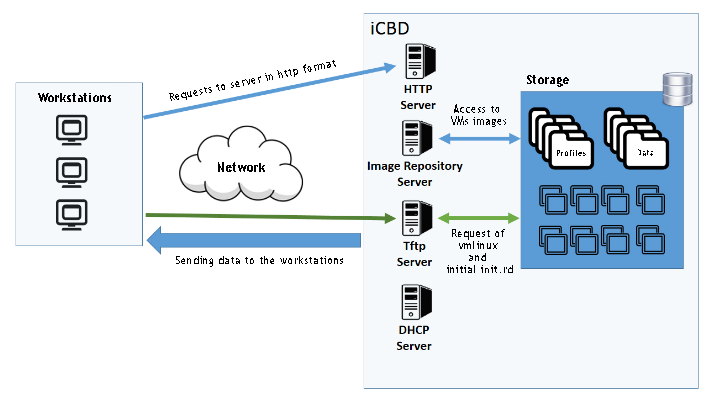
\includegraphics[height=3in]{cap1_icbd}
%    \caption{iCBD architecture. Adapted from \enquote{Linked clones baseados em funcionalidades de snapshot do sistema de ficheiros} by Nuno Alves~\cite{Nuno2016}}
%    \label{fig:icbd}
%\end{figure}

%\newpage

In short, the primary objectives of the project are:

\begin{itemize}
	%
    \item Offering a work environment and experience of use so close to the traditional one that there is no disruption for the users when they begin to use this platform.
    %
    \item Enabling centralised management of the entire infrastructure, including servers, in their multiple roles, storage and network devices, all from a single point.
    %
    \item Completely decouple users and workstations in order to promote mobility.
    %
    \item Support disconnected operation of mobile workstations.
	%
\end{itemize}

When all these objectives are taken into account, there is a clear distinction from other solutions currently (and previously) available. As far as we know, no other solution is so comprehensive in the use of the resources offered by the physical workstations whether they are PCs, laptops or similar devices.


%%-------------------------------------------------------------------
%%	1.3. - Previous Work
%%-------------------------------------------------------------------
\subsection{Previous Work} % (fold)
\label{sub:intro_previous_work}

The iCBD project started about two years ago, and there has been a lot of work in that period, namely by DI-FCT/NOVA students. Previous work was focused on the creation of the instances of virtual machines, using either the storage system’s snapshot mechanisms (for those where native snapshots were available) or the hypervisor’s own mechanism. These studies resulted in two MSc dissertations, one carrying out a more in-depth study of Btrfs (and other file systems) while the other focused itself in object-based storage, particularly on the Ceph (RADOS) product.

These two avenues, file system and object-storage system, proved themselves well suited for the iCBD project, and resulted in the next step, namely on how to support a multi-node, scalable, and failure-tolerant iCBD infrastructure, one where nodes may be geographically dispersed.



%%-------------------------------------------------------------------
%%	1.4 - Problem Stating and Main Contributions
%%-------------------------------------------------------------------
%\section{Problem Stating and Main Contributions} % (fold)
\section{Problem Stating and Main Contributions}
\label{sec:intro_project_contributions}

This dissertation aims to build upon the previous contributions, deeply study the core of the iCBD platform, and tackle the next set of questions, mainly:

\begin{itemize}
	%\item \textit{Needing a distribute data model between nodes, which can be set apart geographically, how to achieve that and maintain the consistency and availability of the data?}
	%\item \textit{How to scale the platform in order to handle a large number of clients and maintain or even enhance the performance?}
	\item \textit{In a geographically dispersed, multi-server iCBD infrastructure, how do we keep the VM templates consistent and available even on the presence of network faults?}
	%
	\item \textit{How do we keep a simple management interface in a distributed platform?}
	%
	\item \textit{How to scale the platform in order to handle a large number of clients and maintain or even enhance its performance?}
	%
\end{itemize}




%%-------------------------------------------------------------------
%%	3.2. - Replication and Caching - The Problem 
%%-------------------------------------------------------------------
\subsection{Replication and Caching - The Problem}
\label{sec:intro_replication_cache_theproblem}

To address the previous questions, we start with a known fact: providing high availability for data requires redundancy, and the simplest way to provide redundancy is to have replicas. Therefore, building a replication mechanism is clearly our starting point. With that in mind, we tackle a second part of the problem: if we want to provide to the iCBD clients (workstations) fast access to the data, that data must be moved, or cached, near those clients. Now, if our cache stores the full data objects that the client needs, and not just parts of those objects, caching becomes just a side-effect from replication.


%\subsection{Motivation and Goals}
\paragraph{Establishing Goals}
\label{par:intro_motivation_goals}

Providing a mechanism that ensures the correct replication of data between nodes of the platform is of paramount importance; but other objectives, such as achieving the best performance possible on data transfer operations – that is, transfer speed must be maximised, and the amount of data moved around should be minimised, and the process should not be computationally intensive – are also important. Another goal is ease of integration of the replication process with multiple technologies: the iCBD storage layer is open to different storage backends – we already mentioned Btrfs and Ceph. So, the design of the replication module should strive for an API that eases the integration with different backend technologies, as long as these do provide a snapshotting mechanism.

As far as caching is concerned, two problems must be addressed: how to plan the number and location of cache (i.e., replica) servers, and which platform services are fundamental for running images on the user’s workstations and how can they be integrated with the replication and caching infrastructure in order to deliver the best possible experience to the highest number of clients.

To summarise, the following list expresses the key requirements that must drive the architecture, design, planning and execution of (the rest of) our work:

\begin{itemize}
	%
    \item The iCBD platform needs to be always available and maintain top-notch performance in multiple locations, while serving a considerable number of clients.
    %
    \item There are two main reasons for data replication: fault-tolerance (replicas represent backups) and moving data closer to the clients.
    %
    \item Taking for granted that data is close to the consumer, devise ways to deliver that data (to the client) as efficiently as possible.
	%
	\item Booting a client should require the smallest number of platform functionalities possible, simplifying the boot process near the consumer.
	%
\end{itemize}

%\subsection{System Overview}
%\label{sub:system_overview}

%\subsection{Requirements}
%\label{sub:requirements}



%%-------------------------------------------------------------------
%%	1.3. - Main Expected Contributions
%%-------------------------------------------------------------------
\subsection{Main Expected Contributions} % (fold)
\label{sub:intro_main_expected_contributions}

The main expected contributions are: 

\begin{itemize}
  %
  \item Perform a throughout analysis of the iCBD platform layers and modules that already implemented, in order to understand its internals, to document it and allow an efficient planning of the remaining of our work. 
  %
  \item Study, develop, and evaluate an implementation of a distributed and replicated storage platform to support VMs, built on top of Btrfs.
  %
  \item Implement a client-side caching solution in order to increase availability, improve response time, and enable better management of resources.
  %
  \item Integrate the solutions described above with the previous work and the existing infrastructure.
  %
  \item And, finally, carry out a series of tests that a) allow us to assert that our replication and caching system is functionally complete and stable enough for production use, b) allows us to draw meaningful conclusions about its performance, and c) provide us with hints for future enhancements of the iCBD platform.
  %
\end{itemize}


%In a more concrete approach, we present the work plan, for achieving the above objectives, distributed by the two main topics.


%\subsubsection{Replication}
%\paragraph{Replication}
%\label{par:intro_replication_goals}
%
%\begin{itemize}
%	\item Create a middleware that integrates with the core functionalities already developed within the iCBD platform.
%	%
%	\item Should aim to be storage provider agnostic (in this thesis work with BTRFS but remain easy to integrate with others).
%	%
%	\item Work with compression algorithms to achieve a lower bandwidth consumption.
%	%
%	\item Be able to use encrypted and unencrypted communications for all data flows. 
%	%
%	\item Capitalize the snapshotting features of the storage layer in order to minimise the volume of data transferred, only sending the differences between versions whenever possible.
%	%
%	\item Provide a simple CLI and a REST API for interacting with the replication module functions.
%\end{itemize}
%
%This subject is further developed in \textbf{Section~\ref{sec:impl_icbdrep}}.
%
%%\subsubsection{Cache Server}
%\paragraph{Caching}
%\label{par:intro_caching_goals}
%
%\begin{itemize}
%	\item Dilute some cost of the infrastructure by having commodity hardware as proximity servers.
%	%
%	\item Bring the data closer to the final clients giving enough storage capacity to servers, storing the most used images.
%	% Provide a good and consistent user experience, with no significant diference in boot time and perceived (OS and APPS) performance between running from a local disk (even an SSD) or from the iCBD Platform
%	%
%	\item Facilitate a user experience where the is no distinction on booting an OS from a local disk or the iCBD platform.
%	%
%	\item Build a completing working iCBD platform on the FCT NOVA campus.
%	%
%	\item Study the benefits of introducing cache servers and the platform performance as a whole, comparing the performance of the system to a traditional OS install base.  
%\end{itemize}
%
%A detailed view of this work is presented in \textbf{Section~\ref{sec:impl_cache_server}}.
% subsection main_expected_contributions (end)



%%-------------------------------------------------------------------
%%	1.5 - Document Structure
%%-------------------------------------------------------------------
\section{Document Structure} % (fold)
\label{sec:intro_document_structure}

The rest of the document is structured as follows:

\begin{itemize}
	%
  \item \textit{Chapter~\ref{cha:research_context}}  \textbf{Research Context} - This chapter presents existing technologies and theoretical approaches which were studied; examples include storage systems and their features, and details on virtualisation techniques and hypervisors.
	%
  \item \textit{Chapter~\ref{cha:icbd}} \textbf{iCBD - Infrastructure for Client-Based Desktop} - In this chapter, we present the iCBD platform: we start with an overview of the solution, describe the multiple layers and try to explain the conceptual and architectural decisions that were made. This chapter is essential to the understanding of the bigger picture and where our work fits in.
  %
  \item \textit{Chapter~\ref{cha:impl_replication_caching}} \textbf{Implementation of the \textit{iCBD-Replication and Cache Server}} - We start with an in-depth view of the implementation of the iCBD Replication module, detailing the architectural decisions and the implemented components. Then, a description is given on the efforts to build, on the FCT NOVA campus, a server infrastructure exclusively dedicated to the iCBD project. Then we explain how to build and deploy the iCBD Cache Server software for a node that will support a student’s computer lab with 15 workstations in the Computer Science Department.
  %
  \item \textit{Chapter~\ref{cha:evaluation}} \textbf{Evaluation} - In this chapter, we present the evaluation process employed to validate our Implementation, with an emphasis on the analysis of the results we obtained and a comparison with the baseline values.
  %
  \item \textit{Chapter~\ref{cha:conclusion}} \textbf{Conclusions \& Future Work} - This chapter concludes the dissertation; we provide the answers to the questions we raised in the Introduction, summarise the results achieved in the evaluation process, and recall some ideas for further improvements, ones that were formulated during the implementation process, and we believe are a good starting point for future work.
  %
\end{itemize}

% section document_structure (end)
